\documentclass[a4paper]{article}

\usepackage[margin=2.5cm]{geometry}
\usepackage[pdftex]{graphicx}
\usepackage[utf8]{inputenc}
\usepackage[T1]{fontenc}
\usepackage{textcomp}
\usepackage{babel}
\usepackage{amsmath, amssymb, amsthm}
\usepackage[colorlinks=true,linkcolor=blue]{hyperref}
\usepackage{float}
\usepackage{mathrsfs}
%\usepackage{enumitem}
%% for identity function 1:
\usepackage{bbm}
%%For category theory diagrams:
\usepackage{tikz-cd}
%%For code (e.g. python) in latex:
%\usepackage{listings}
%
%Usage: 
%\begin{lstlisting}[language=Python]
%\end{lstlisting}

\newcommand{\incfig}[2][1]{%
\def\svgwidth{#1\columnwidth}
\import{./figures/}{#2.pdf_tex}
}


\theoremstyle{plain}% default
\newtheorem{theorem}{Theorem}[section]
\newtheorem{lemma}[theorem]{Lemma}
\newtheorem{proposition}[theorem]{Proposition}
\newtheorem*{corollary}{Corollary}


\theoremstyle{definition}
\newtheorem{defn}{Definition}[section]
\newtheorem{example}{Example}[section]
\newtheorem{exercise}[example]{Exercise}
\newtheorem{problem}[example]{Problem}


\theoremstyle{remark}
\newtheorem*{remark}{Remark}
\newtheorem*{note}{Note}






% figure support
\usepackage{import}
\usepackage{xifthen}
\pdfminorversion=7
\usepackage{pdfpages}
\usepackage{transparent}

\pdfsuppresswarningpagegroup=1

\setlength\parindent{0pt}

\newcommand{\qedwhite}{\hfill \ensuremath{\Box}}

%Inequalities
\newcommand{\cycsum}{\sum_{\mathrm{cyc}}}
\newcommand{\symsum}{\sum_{\mathrm{sym}}}
\newcommand{\cycprod}{\prod_{\mathrm{cyc}}}
\newcommand{\symprod}{\prod_{\mathrm{sym}}}

%Linear Algebra

\DeclareMathOperator{\Span}{span}
\DeclareMathOperator{\Ima}{Im}
\DeclareMathOperator{\diag}{diag}
\DeclareMathOperator{\Ker}{Ker}
\DeclareMathOperator{\ob}{ob}
\DeclareMathOperator{\Hom}{Hom}
\DeclareMathOperator{\sk}{sk}
\DeclareMathOperator{\Vect}{Vect}
\DeclareMathOperator{\Set}{Set}
\DeclareMathOperator{\Group}{Group}
\DeclareMathOperator{\Ring}{Ring}
\DeclareMathOperator{\Ab}{Ab}
\DeclareMathOperator{\Top}{Top}
\DeclareMathOperator{\Htpy}{Htpy}
\DeclareMathOperator{\Cat}{Cat}
\DeclareMathOperator{\CAT}{CAT}
\DeclareMathOperator{\Cone}{Cone}

\DeclareMathOperator{\dist}{dist}

%Row operations
\newcommand{\elem}[1]{% elementary operations
\xrightarrow{\substack{#1}}%
}

\newcommand{\lelem}[1]{% elementary operations (left alignment)
\xrightarrow{\begin{subarray}{l}#1\end{subarray}}%
}

%SS
\DeclareMathOperator{\supp}{supp}
\DeclareMathOperator{\Var}{Var}

%NT
\DeclareMathOperator{\ord}{ord}

%Alg
\DeclareMathOperator{\Rad}{Rad}
\DeclareMathOperator{\Jac}{Jac}

\DeclareMathAlphabet{\pazocal}{OMS}{zplm}{m}{n}
\newcommand{\unif}{\pazocal{U}}

\title{A brief introduction to algebraic topology}
\date{}
\author{Jonas Trepiakas}

\begin{document}
\maketitle

\textit{Prerequisites:} Basic topology for a few of the preliminary proofs, but
I will try to convey most things visually so that we won't get caught up in
technicalities on the topological side.\\
\linebreak


The goal is to get a basic visual understanding of fundamental things in
algebraic topology such as path homotopies and the homotopy-lifting lemma, get
a visual understanding of why $\pi_1 (S^{1}) \cong \mathbb{Z}$, and then work
on
and hopefully solve the following problem:
\begin{center}
    Let $A_1, A_2, A_3$ be closed\footnote{A subset $A$ of
    $\mathbb{R}^3$ is closed if for any
$x \in \mathbb{R}^3 - A$, there exists some $\varepsilon >0$ such that
$B(x,\varepsilon) \subset \mathbb{R}^3 - A$, i.e., such that the ball with
center $x$ and radius $\varepsilon$ is contained in the complement of
$A$.} and bounded\footnote{A subset
    $A$ of $\mathbb{R}^3$ is bounded if there exists some
    $R \in \mathbb{R}$ such that
for any $x,y \in A$, we have 
$\dist(x,y) \le R$.} sets in $\mathbb{R}^3$. Prove that there is one plane
$P \subset \mathbb{R}^3$ that simultaneously divides each
$A_{i}$ into two pieces of equal measure.
\end{center}


To show this, we wish to show the Borsuk-Ulam theorem in two dimensions aka
the
there-must-exist-a-pair-of-antipodal-points-on-earth-having-the-same-temperature
theorem:\\
\linebreak
\textbf{Theorem. (Borsuk-Ulam)}\textit{
    For every continuous map $f  \colon S^2 \to \mathbb{R}^2$ there exists
    a pair of antipodal points $x$ and $-x$ in $S^2$ with
$f(x) = f(-x)$.\footnote{$S^{n}$ is the $n$-sphere $S^{n} := 
\left\{ x \in \mathbb{R}^{n+1}  \colon \|x \|=1 \right\} $}}
\subsection*{Warm-up for people who don't know much group theory}
    Algebraic topology is about using algebra to describe topological objects,
    so to warm up, try the following exercise.\\
    \linebreak
\textbf{Exercise.} Choose your favorite conic and let $G$ denote the set of
points of the conic. Now choose a point which we will call $0$ in $G$. Then we
define a binary operation as follows: for any points $A,B \in G$, we define $A
* B$ as the point of intersection between the conic and the line parallel to
$AB$ passing through $0$. Show that $(G,*)$ is a group.

\subsection*{Paths and Homotopy}

\textbf{Definition.} A \textbf{path} in a space $X$ is a continuous map
$f  \colon I \to X$ where $ I = \left[ 0,1 \right] $.\\
\linebreak
\textbf{Definition.} A \textbf{homotopy} of paths in $X$ is a continuous map
$F  \colon I \times I \to X$ such that $F(0,t) = x_0$ and $F(1,t) = x_1$ for
all $t \in I$.\\
When two paths $f_0(x) = F(x,0)$ and $f_1(x) = F(x,1)$ are connected in this way by a homotopy
$F$, they are said to be \textbf{homotopic}, and we denote this
by $f_0 \simeq f_1$.

\begin{figure}[H]
    \centering
    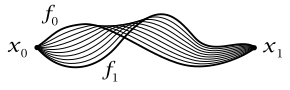
\includegraphics[width=0.3\textwidth]{homotopy.png}
    \caption{Here is an example of what a homotopy of paths could look like.}
    \label{fig:homotopy-png}
\end{figure}

\textbf{Exercise 1.} Suppose we take any two paths
$f_0$ and $f_1$ in $\mathbb{R}^{n}$ having the same endpoints $x_0$ and $x_1$.
Show that they are homotopic.\\
\linebreak
\textbf{Exercise 2.} Show that the relation of homotopy on paths with fixed
endpoints in any space is an equivalence relation.\\
\linebreak
Thus we can denote the equivalence class of a path $f$ under the equivalence
relation of homotopy by $\left[ f \right] $, which will be called the
\textbf{homotopy class} of $f$.\\
So in figure 1 above, we would thus have $\left[ f_0 \right] = \left[ f_1
\right] $.\\
\linebreak
We wish to look at loops, i.e., paths with the same start and end point, and
show that the set of homotopy classes of loops with a fixed start and end point
has a group structure. For this, we need to define the group operation:\\


\textbf{Definition.} Given two paths $f,g  \colon I \to X$ such that
$f(1) = g(0)$, we can define a concatenation of the paths
$f \cdot g$ by
\[
f \cdot  g (s) = \begin{cases}
    f(2s), & 0 \le s \le \frac{1}{2}\\
    g(2s-1), & \frac{1}{2} \le s \le 1
\end{cases}.
\] 
This path traverses $f$ during $\left[ 0,\frac{1}{2} \right] $ and then
traverses $g$ during $\left[ \frac{1}{2},1 \right]$.\\
\linebreak
Suppose we restrict our attention to paths
$f  \colon I \to X$ with the same start and end point, $f(0) = f(1) = x_0 \in
X$. Such paths are called \textbf{loops}, and $x_0$ is called the
\textbf{basepoint}. The set of homotopy classes $\left[ f \right] $ of loops
$f  \colon I \to X$ at the basepoint $x_0$ is denoted by
$\pi_1 (X,x_0)$.\\
\linebreak
Algebraic topology makes use of algebra to describe topological objects, so to
warm up, let's look at how we can attribute a group to any conic.\\
\linebreak
\textbf{Proposition.} $\pi_1(X,x_0)$ is a group with respect to the product
$\left[ f \right] \left[ g \right] =
\left[ f \cdot g \right] $.\\
$\pi_1 (X,x_0)$ is called the \textbf{fundamental group} of $X$ at the
basepoint
$x_0$.\\
\linebreak


\textbf{Exercise 3.} Show that $\pi_1 (\mathbb{R}^{n},x_0) \cong 0$ for any
$x_0 \in \mathbb{R}^{n}$ where $0$ is the trivial group.




\subsection*{Lifting homotopies}
\textbf{Definition.}
    Given a map $f  \colon X \to Y$ and a map $g  \colon Z \to Y$, a 
    \textbf{lift} of $f$ to $Z$ is a map
    $h  \colon X \to Z$ such that $f = g \circ h$. We say that
    $f$ factors through $h$.\\
    We can also state this by saying that the following diagram commutes
    \begin{equation*}
    \begin{tikzcd}
        & Z \ar[d, "g"]\\
        X \ar[ru, "h"] \ar[r, "f"] & Y
    \end{tikzcd}
    \end{equation*}
    
\textbf{Homotopy-lifting lemma.}
    \textit{If $F  \colon I \times I \to S^{1}$ is a map such that
    $F(0,t) = F(1,t) = 1$ for $0 \le t \le 1$, there exists a unique
    map $\tilde{F}  \colon I \times I \to \mathbb{R}$ such that
    $\tilde{F}$ is a lift of $F$ and
    \[
    \tilde{F}(0,t) = 0, \, 0 \le t \le 1.
    \] 
}
This lemma can be encapsulated by stating that the following diagram commutes:

\begin{equation*}
\begin{tikzcd}
    \left\{ 0 \right\} \times I \ar[r, "0"] \ar[d, "\iota", hookrightarrow]
    & \mathbb{R} \ar[d, "\pi"]\\
    I \times I \ar[ru, " \exists ! \tilde{F}", dotted] \ar[r, "F"] & S^{1}
\end{tikzcd}
\end{equation*}




\subsection*{All the fun stuff}

\textbf{Theorem.} $\pi_1 (S^{1})$ is an infinite cyclic group generated by the
homotopy class of the loop $\omega (s) = \left( \cos 2 \pi s, \sin 2 \pi
s \right) $ based at $(1,0)$. I.e., $\pi_1 (S^{1}) \cong \mathbb{Z}$.\\
\linebreak





\textbf{Exercise 4.} 
Suppose the Borsuk-Ulam theorem is false for $f  \colon S^2 \to \mathbb{R}^2$.
Try to create a map $g$ using $f$ that maps into $S^{1}$ and look at how the image
of the equator of $S^2$ under $g$ behaves.\\
    \linebreak
    \textbf{Definition.} A path $f  \colon I \to X$ is said to be
    \textbf{nullhomotopic} if it is homotopic to a constant map
    $c  \colon I \to X$, i.e. $f \simeq c$ and $c(t) = c(0)$ for all $t \in
    I$.\\
    \linebreak
    \textbf{Exercise 5.} Find a non-trivial loop in the image of $g$ which is
    also nullhomotopic, thus giving a contradiction.\\
    \linebreak
\textbf{Problem:} Prove the original problem using the Borsuk-Ulam theorem.\\
\linebreak

\textbf{Extra problem:} Also prove the following problem: Whenever $S^2$ is expressed
as the union of three closed sets $A_1, A_2$ and $A_3$, then at least one of
these sets must contain a pair of antipodal points $\left\{ x,-x \right\} $.
Show that $3$ in this result is the best possible.\\
\linebreak
\textbf{Extra exercise.} Does the Borsuk-Ulam theorem hold for the torus? In
other words, for every map $f  \colon S^{1} \times S^{1} \to \mathbb{R}^2$ must
there exist $(x,y) \in S^{1} \times S^{1}$ such that $f(x,y) = f(-x,-y)$?


\subsection*{Extra chapter for fun - induced homomorphisms}
\textbf{Definition.} A map $r  \colon X \to X$ such that
$r(X) = A$ and $r |_{A} = \mathbbm{1}$ for a subspace $A \subset X$ is called
a retraction.\\
\linebreak
\textbf{Definition.} A \textbf{deformation retraction} of a space $X$ onto
a subspace $A$ is a continuous map $F  \colon X \times I \to X$ such that
$F(x,0) = \mathbbm{1}$ and $F(X,1) = A$ and
$F(x,t) = x$ for all $x \in A$ and $t \in I$.\\
\linebreak



Suppose now $\varphi  \colon X \to Y$ is a map taking the basepoint $x_0 \in X$
to the basepoint $y_0 \in Y$. WRite this as $\varphi  \colon (X,x_0) \to
(Y,y_0)$. Then $\varphi$ induces a homomorphism
$\varphi_{*}  \colon \pi_1 (X, x_0) \to \pi_1 (Y,y_0)$ by
$\varphi_* \left[ f \right] = \left[ \varphi \circ f \right] $ for any loop
$f  \colon I \to X$ based at $x_0$.\\
\linebreak
\textbf{Exercise.} Convince yourself that $\pi_1$ is a functor.\\
\linebreak
\textbf{Proposition.} If a space $X$ retracts onto a subspace $A$, then the
homomorphism $\iota_{*}  \colon \pi_1(A,x_0) \to \pi_1 (X,x_0)$ induces by the
inclusion $\iota  \colon A \hookrightarrow X$ is injective. If $A$ is
a deformation retract of $X$, then $\iota_*$ is an isomorphism.\\
\linebreak
\textbf{Proposition.} $\pi_1 (X\times Y) \cong \pi_1(X) \cong \pi_1(Y)$ if $X$
and $Y$ are path-connected.\\
\linebreak
\textbf{Problems.} Show that there are no retractions $r  \colon X \to A$ in
the following cases:\\
\begin{enumerate}
    \item $X = \mathbb{R}^3$ with $A$ any subspace homeomorphic to $S^{1}$.
    \item $X = S^{1} \times D^2$ with $A$ its boundary torus $S^{1} \times S^{1}$
    \item $X$ the Möbius band and $A$ its boundary circle.
\end{enumerate}

\textbf{Problem.} Let $X \subset \mathbb{R}^3$ be the union of $n$ lines
through the origin. Compute $\pi_1 \left( \mathbb{R}^3 - X \right) $.\\
(You may
use the fact that $\pi_1 \left( \bigvee_{i = 1}^{n} S_i^{1} \right) =
\bigoplus_{i = 1}^{n} \mathbb{Z}$ where $\bigvee_{i=1}^{n}S_i^{1}$ denotes
the one-point union of $n$ circles - i.e., $n$ circles joined at a single
point.




    
\end{document}
